\section{Contexto}\label{contextualizacao}


A tomada de decisão baseada em evidências é um dos princípios fundamentais de gestão da qualidade definido na norma \citeonline{iso9000}. A ISO9000 destaca como este princípio é essencial para a gestão da qualidade de um produto, contribuindo para a tomada de decisões técnicas e gerenciais eficazes. Já a norma \citeonline{iso25010}, evolução da \citeonline{iso9126}, é específica para avaliação de requisitos de qualidade de software e sistemas. Ela foca nos aspectos da qualidade do produto, que inclui aspectos da visão da qualidade em uso. 

Nas normas \citeonline{iso9126} e \citeonline{iso25010}, os aspectos da qualidade de \textit{software} são descritos em um modelo hierárquico em termos de características e suas respectivas subcaracterísticas. A criação de ambas foi profundamente influenciada pelos modelos de McCall \cite{mccall1977factors} e Boehm \cite{boehm1978characteristics}, que foram pioneiros na caracterização e no fornecimento de visões estruturadas e hierárquicas da qualidade de \textit{software}.

% ------------
% comecei a falar sobre os modelos aqui mas senti que poderia me alongar sem necessidade, acabei optando por citar o seu pioneirismo e como influenciaram as isos, caso não seja o suficiente favor me informar.
% ------------
% O modelo de \citeonline{mccall1977factors} foi um dos precussores no fornecimento de uma visão estruturada da qualidade de \textit{software} e e foca nos aspectos de operação, revisão e transição do produto, características mais externas e observáveis do \textit{software}. Já o modelo de \citeonline{boehm1978characteristics} provê uma visão detalhada e hierárquica, propondo características em três camadas, de alto, intermediário e baixo nível. Ambos os modelos são apresentados nas Figuras \ref{fig:mccall} e \ref{fig:boehm}.

Dentre as características definidas na visão da  qualidade em uso, destaca-se a eficácia, que seria a acurácia e a completude com as quais os usuários alcançam seus objetivos (vide Figura \ref{fig:quality-in-use}). No entanto, apesar de fornecer essas definições, a ISO não propõe um modelo para medir ou avaliar as características de forma quantitativa, o que impede sua aplicação de forma direta. Assim, se torna necessária a combinação desta com outras teorias e modelos de referência.

Um modelo de referência existente é a norma \citeonline{iso9241}, que trata das características e subcaracterísticas de usabilidade, dentre elas a eficácia. A ISO define que, para se avaliar esta característica, é necessária a definição de métricas que possam representar a completude com a qual o produto permite que o usuário realize as tarefas desejadas durante sua utilização.

No contexto de avaliação da qualidade de um produto, uma prática comum é a de coleta de \textit{feedbacks}. Contudo, esse processo pode ser demorado e muitas vezes não fornecer informações suficientes para a tomada de decisões assertivas \cite{olsson_opinions_2014}. Além disso, com a consolidação da cultura de desenvolvimento orientada à práticas ágeis e do pensamento \textit{Lean}, empresas de tecnologia passaram a adotar práticas que diminuíram o período de disponibilização de \textit{releases} e tornaram essa atividade contínua e frequente \cite{kevic_characterizing_2017}.

A metodologia \textit{Lean} provê um guia para a combinação de \textit{design}, desenvolvimento e validação agregados em um ciclo de descoberta e entrega de valor \cite{fagerholm_right_2017}. Esta abordagem influenciou o desenvolvimento de \textit{software} e diversas práticas passaram a ser adotadas para que o mesmo se tornasse uma realidade, como a Integração e a Entrega Contínuas \cite{fitzgerald2015continuous}.

Essas e outras práticas se consolidaram no desenvolvimento de \textit{software} de código aberto, com o objetivo de "liberar cedo e frequentemente" \cite{feller2005perspectives}. Esse pensamento se alinha aos princípios \textit{Lean} de aprendizado contínuo e contribuiu para o estabelecimento de práticas que garantem a flexibilidade e rápida adaptação exigidas pelos ambientes ágeis de desenvolvimento \cite{fitzgerald2015continuous}.

Nesse cenário de desenvolvimento contínuo e falta de formalização de mecanismos de coleta de \textit{feedback}, aumenta-se o risco de desalinhamento do produto com as necessidades dos usuários durante a construção de novas funcionalidades \cite{olsson2013data}. E é nestas circunstâncias que surge a chamada Experimentação Contínua, uma abordagem de desenvolvimento que sistematiza a escolha entre duas versões de produto, baseando-se no resultado de testes de hipóteses estatísticas provenientes da coleta de métricas de uso real do \textit{software}.

A Experimentação Contínua tem se tornado um padrão nas grandes empresas de tecnologia \cite{kohavi_seven_2014}. Contudo, a área ainda carece de consenso de uma taxonomia ou corpo de conhecimento bem definido sobre processos, ferramentas, definições ou estratégias \cite{erthal_characterization_2023}.

% \begin{figure}[h]
% \centering
% \caption{Características da Qualidade em Uso}
% 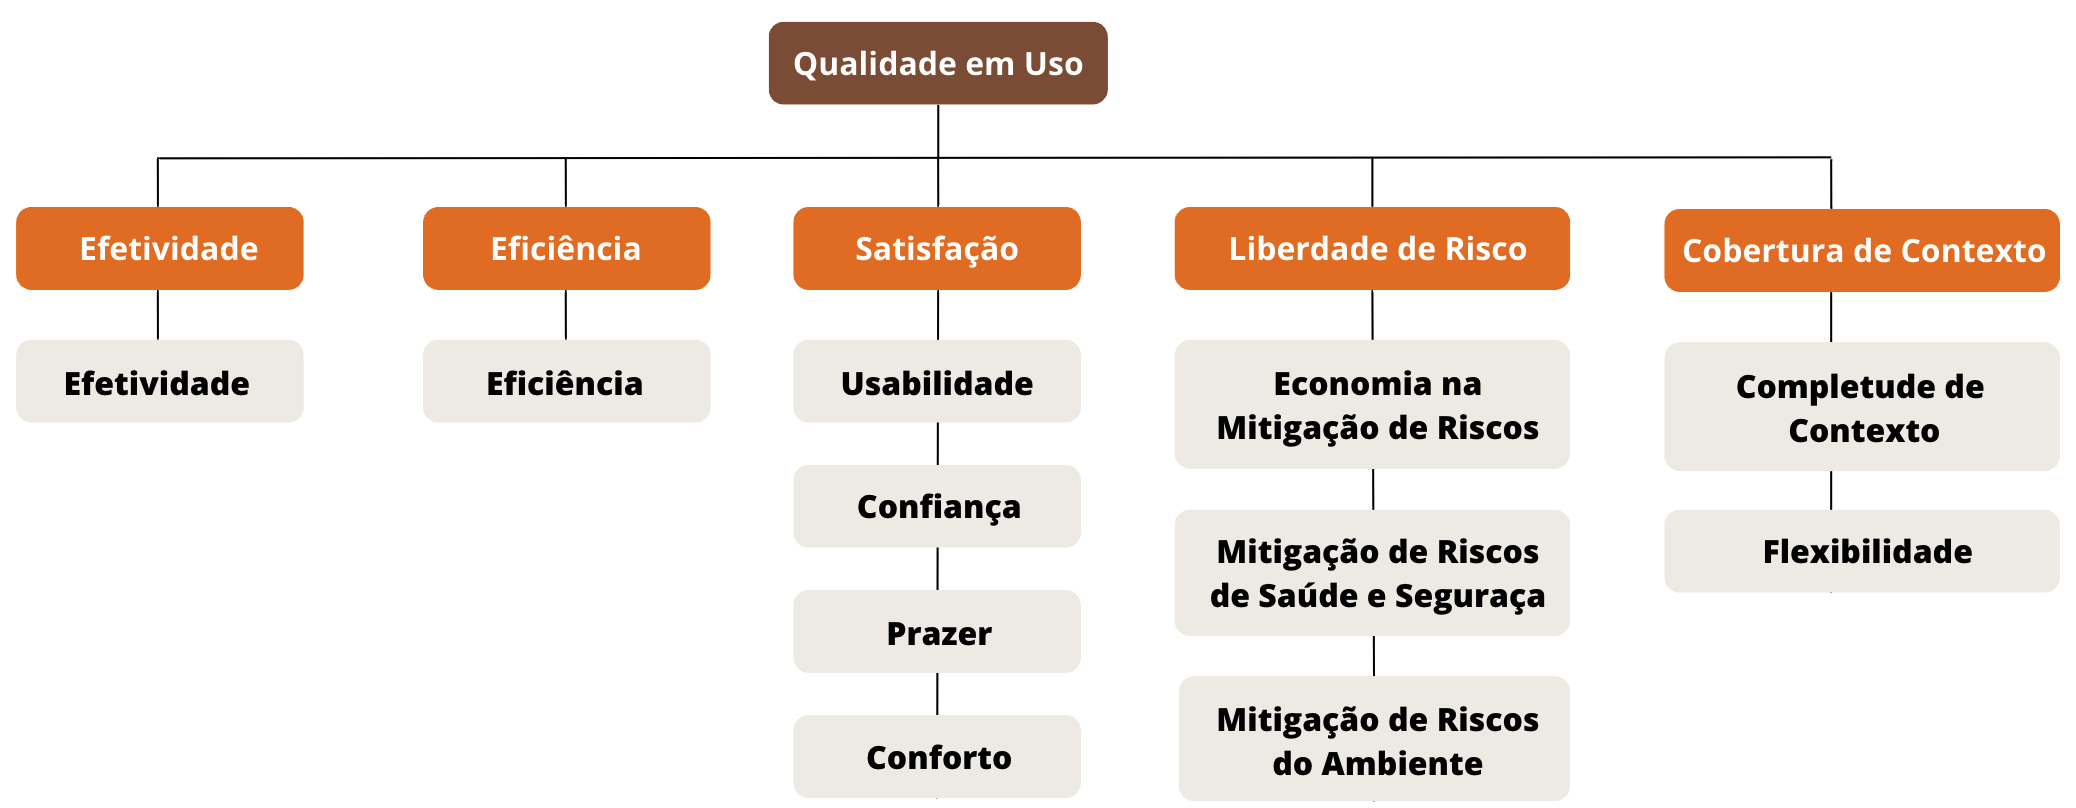
\includegraphics[width=1\linewidth]{figuras/quality_in_use.png}
% \text Fonte: Adaptado da Norma \citeonline{iso25010}
% \label{fig:model-quality-in-use}
% \end{figure}